\documentclass[aps,pra,10pt,floatfix,nofootinbib]{revtex4-1}

\usepackage{bbm}
\usepackage{amsmath}
\usepackage{amssymb}
\usepackage{graphicx}
\usepackage{amsfonts}
\usepackage{amsthm}
\usepackage{tikz}

\newtheorem{thm}{Theorem}[section]
\newtheorem{cor}[thm]{Corollary}
\newtheorem{lem}[thm]{Lemma}
\newtheorem{prop}[thm]{Proposition}

\theoremstyle{definition}
\newtheorem{defn}[thm]{Definition}
\newtheorem*{assump1}{Classical assumption}
\newtheorem*{assump2}{Determinism and Reversibility assumption}

\begin{document}
	
\section{What is information entropy?}

TL;DR .

Starting from the 1950s, the connection between information theory and thermodynamics has been increasingly made clear. What I believe is still largely unnoticed is that there is a deep link between information theory and Hamiltonian mechanics as well. I want to explore this link in the next few posts and it is appropriate to first have a clear idea on what information entropy is.

The concept of entropy in physics is unfortunately associated with a certain amount of vagueness. While mathematically is well defined, I have never heard a crisp conceptual understanding (e.g. it measures "disorder", it has to do with how much the system is homogeneous, ...). Entropy in information theory, or Shannon's entropy, instead has a crisp intuitive meaning and therefore I cringe when I hear physicists defining it as "lack of information" or any other vague description. So, let's see if we do better.

The scenario is this: you have a distribution over a set of possibilities. You pick an element according to that distribution. On average, how many bits of information you have to use to tell me which element have you picked? How many one-zeros? How many yes-no answers? If that doesn't make sense yet, hopefully it will after we go through a few examples.

\section{Examples}

Suppose you have a bag with 40 balls. 20 are green and 20 are red. Suppose you pick a ball and I want to know the color. Suppose I can only ask you yes or no questions. How many questions do I have to ask you? One suffices: "Is it red?". If the answer is yes, I know it's red, if the answer is no, I know it's green. We can rephrase by asking: how many one-zero choices? That is: how many bits of information you need to give me? The answer is one bit: 0 for green and 1 for red. That is: all the information can be encoded into one zero-one choice.

Let's do it again in another case. Suppose all 40 balls are green. How many bits of information? The answer is zero bits: I already know you are going to get a green ball.

Suppose there are 10 balls for each of these color: green, red, yellow and blue. How many bits of information? We can set 00 for green, 01 for red, 10 for yellow and 11 for blue. That is two zero-one choices: it's two bits of information.

Shannon's entropy simply generalizes this idea: given a $n$ cases each with a probability $p_i$, the average number of bits (i.e. yes/no questions) required to identify an element is:

\begin{equation}
\label{ShannonEntropy}
H(p_1, ..., p_n) = - \sum_{i=1}^{n} p_i \log p_i
\end{equation}

The base of the logarithm determines the units. If it's base $2$, then we are using bits. But sometimes is useful to use base $e$ (i.e. the natural log) since it has nice properties. In that case we are using nats, and we have $1$ bit = $\ln 2$ nats.

\section{Uniqueness of the expression}

It is important to understand that the above expression for entropy is not arbitrary. Consider the following three requirements.

\begin{enumerate}
	\item $H(p_1, ..., p_n)$ is continuous.
	\item $H(p_1, ..., p_n)$ increases if the number of choice increases. That is, suppose you have two uniform distributions over $n$ and $m$ cases respectively. If $m>n$ then $H(\frac{1}{m}, ..., \frac{1}{m})>H(\frac{1}{n}, ..., \frac{1}{n})$.
	\item $H(p_1, ..., p_n)$ does not change if we group/break down choices. Consider the following trees:
	\begin{figure}[h]
	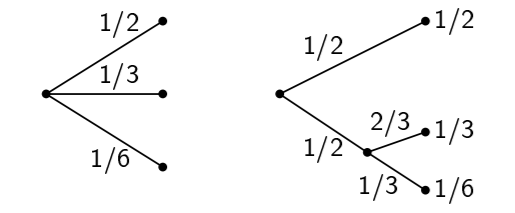
\includegraphics[scale=0.50]{ShannonTree}
	\centering
	\end{figure}
	
	We should get the same result whether we have one distribution or we combine the two. That is: $H(\frac{1}{2}, \frac{1}{3}, \frac{1}{6}) = H(\frac{1}{2},\frac{1}{2}) + \frac{1}{2} H(\frac{2}{3}, \frac{1}{3})$. The coefficient $\frac{1}{2}$ appears because the second choice only occurs half the times.
\end{enumerate}

These are basic requirements that an expression that measures information needs to satisfy. It's not just that Shannon's entropy \eqref{ShannonEntropy} satisfies these conditions: it is the only one that does. Shannon's entropy is not just an expression that we use because it's convenient or because it's known to work: it's the only one that can work.

While we are not going to derive it here, the derivation is not particularly insightful, we can still understand why it is what it is. If a particular case is a choice among $n$ equal cases, it's probability is $p_i=\frac{1}{n}$ and the number of yes/no questions we have to make to get to it is $\log_2 n = \log_2 \frac{1}{p_i} = - \log_2 p_i$. So, when that particular case is selected, we need $- \log_2 p_i$ bits. Now we take the expectation, the average over all cases, and we have $H(p_1, ..., p_n) = - \sum_{i=1}^{n} p_i \log p_i$. We now have the average value of yes/no questions (i.e. bits) needed to identify an element in the distribution.

\section{Relation to physics}

There are a couple of aspects we need to clarify as it allows to understand why such concept is interesting for physics.

First of all, information entropy has nothing to do with knowledge (e.g. what we know about the system or what can be known). This misunderstanding arises because the concept can be applied to probability distribution that represent our knowledge of the system, and in some cases it may relate to knowledge. For example, if there are four boxes and I do not know in which one the ball is hiding, I have a uniform distribution on four cases which has 2 bits of information entropy. Conversely, if I know where it is, the entropy is 0 bits. So, in this more entropy correspond to less knowledge. But this idea does no generalize.

Suppose you have equal confidence that you may or may not win a prize. That is 50\% chance you get one million dollars and 50\% chance you get nothing. That is one bit of information entropy. On the other hand, suppose you know you won a prize but you do not know how much. 50\% chance you won half a million dollars and 50 \% chance you won a million dollars. It is still one bit of information entropy. Yet, I would argue, you know more in the second case: you know you have half a million dollars you can spend right away.

Moreover, not all distributions represent knowledge and/or are statistical. For example, we could have a mass distribution in space. In this case, information entropy does not equate to lack of knowledge. Our knowledge of the mass distribution is perfect: we know exactly how it is spread over a region. The information entropy of a mass distribution in space is as much a physical property of the system as it is the mass distribution itself and it tells us how many bits are necessary to identify the position of a part of the system. Unlike the previous case, this is an objective number. It is this second use that is the most relevant to physics. Nature does not much care about our knowledge: it cares about objective facts.

Another thing to keep in mind is that information entropy is a quantity that relates two levels of description: the distribution and the elements over which the distribution is defined. It is this property that makes it important in physics. This is exactly the same for the thermodynamic entropy, which relates the state of the whole system (i.e. the macro-state) with the state of its components (i.e. the micro-states). For Hamiltonian mechanics, we will study the evolution of distributions over position and momentum and see how it relates to the evolution of particles. Note that other types of entropy (e.g. topological entropy, algebraic entropy) do not have this property and still do not quite understand what they actually quantify.

\section{Conclusion}

This hopefully helps you understand what information entropy measures: how many bits of informations are required on average to identify an element in a distribution. Not "knowledge" or "lack of information" or "disorder" or any other vague concept. In the end, information entropy is a number: to understand it you need to understand what that number quantifies.

\end{document}
